\chapter{交互实验}


\section{实验设计}
我们通过朋友圈,海报招募\ref{fig:poster}已经问卷星的样本服务,招募了100左右的用户。
\begin{figure}
    \centering
    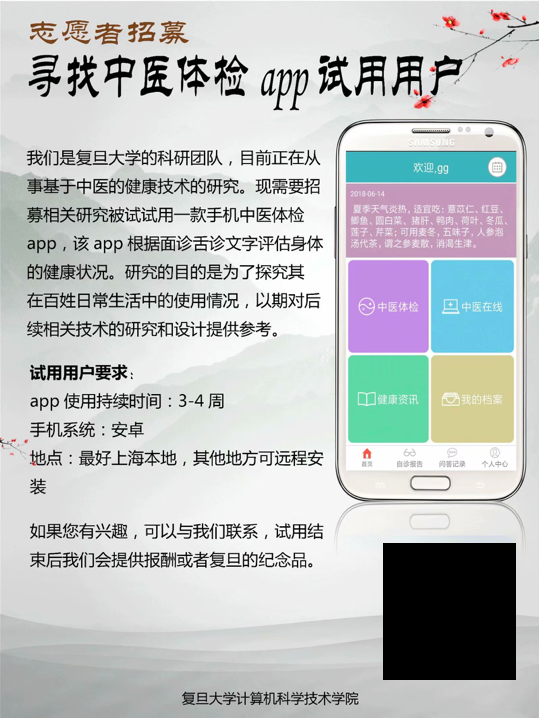
\includegraphics{images/poster.png}
    \caption{招募海报}
    \label{fig:poster}
\end{figure}
\subsection{实验流程}
每个用户的实验流程如下:

1. 用户通过扫描二维码,或者通过我们给定的链接,进入问卷星调查问卷。
2. 完成调查问卷之后,自动进入云中医在线app。通过调用问卷星提供的企业用户接口, 同时把问卷星的问卷id传给云中医在线应用。
3. 在用户完成一次面诊之后,会在健康诊断页面下,看到一个跳转链接,可以选择填写用后问卷。

因此,每个用户在参与实验之后,我们可以得到调查问卷的数据,云中医的使用日志,已经用后问卷的数据。三份数据可以通过问卷id和用户id链接起来,得到特征如表所示。




\section{实验结果}




